%% libcqops — LAB REPORT
%%
%% APPEND-ONLY. One file per session under sessions/, \input in order below.
%% A committed entry is NEVER edited; a correction is a NEW entry carrying
%% \supersedes. Build with `make labreport` (the PDF is gitignored — the .tex
%% is the artefact, the PDF is a build product).
%%
%% To add an entry:  python3 tools/labreport/new_entry.py --title "..."
%%                   then add one \input line at the END of the list below.

\documentclass[11pt,a4paper]{article}
%% libcqops lab report — shared preamble.
%%
%% Everything here is presentation. NOTHING in this file may carry a project
%% fact: a figure, a count, a status. Facts live in the entries, each scoped to
%% the SHA in its own generated header.

\usepackage[a4paper,margin=28mm,headsep=8mm]{geometry}
\usepackage[T1]{fontenc}
\usepackage[utf8]{inputenc}
\usepackage{textcomp}
\usepackage{lmodern}
\usepackage{amsmath}
\usepackage{amssymb}
\usepackage{microtype}
%% `\caption*` is the caption package's, not the article class's — without it
%% LaTeX numbers the float and typesets a literal `*`. Every figure here is
%% unnumbered on purpose: an entry is short, and a cross-reference into another
%% entry would break append-only anyway.
\usepackage[font=small,labelformat=empty,skip=6pt]{caption}
\usepackage{booktabs}
\usepackage{longtable}
\usepackage{array}
\usepackage{enumitem}
\usepackage{xcolor}
%% [H] — figures stay where they are written. A floated figure in a two-page
%% entry lands on a page of its own and reads as belonging to nothing.
\usepackage{float}
\usepackage{tikz}
\usepackage{pgfplots}
\usepackage{fancyhdr}
\usepackage{titlesec}
\usepackage[hidelinks]{hyperref}
\pgfplotsset{compat=1.18}
\usetikzlibrary{positioning,fit,backgrounds}

\definecolor{cqrule}{gray}{0.62}
\definecolor{cqsoft}{gray}{0.35}
\definecolor{cqbg}{gray}{0.955}
\definecolor{cqaccent}{HTML}{1F4E79}

\hypersetup{colorlinks=false,pdftitle={libcqops lab report}}

%% ---- Page furniture ------------------------------------------------------
\pagestyle{fancy}
\fancyhf{}
\renewcommand{\headrulewidth}{0.4pt}
\renewcommand{\footrulewidth}{0pt}
\fancyhead[L]{\footnotesize\color{cqsoft}\textsc{libcqops lab report}}
\fancyhead[R]{\footnotesize\color{cqsoft}\leftmark}
\fancyfoot[C]{\footnotesize\color{cqsoft}\thepage}

\titleformat{\section}{\large\bfseries\color{cqaccent}}{}{0pt}{}
\titlespacing*{\section}{0pt}{20pt}{6pt}

%% ---- An entry ------------------------------------------------------------
%% \entry{number}{date}{title}
\newcommand{\entry}[3]{%
  \clearpage
  \section*{Entry~#1 \,\textcolor{cqrule}{\textbar}\, #2 \,\textcolor{cqrule}{\textbar}\, #3}%
  \markboth{Entry~#1 \textperiodcentered\ #2}{Entry~#1 \textperiodcentered\ #2}%
  \addcontentsline{toc}{section}{Entry~#1 \textperiodcentered\ #2 \textperiodcentered\ #3}%
  \vspace{-2pt}\textcolor{cqrule}{\hrule height 0.8pt}\vspace{10pt}%
}

%% A correction to an earlier entry. NEVER edit the entry itself — a rendered
%% PDF is not something anyone diffs, so a silent change is invisible drift.
%% \supersedes{entry number}{which field}
\newcommand{\supersedes}[2]{%
  \par\noindent\colorbox{cqbg}{%
    \begin{minipage}{\dimexpr\linewidth-2\fboxsep}
      \small\textbf{Supersedes Entry~#1, \emph{#2}.}\ %
      That entry stands as written; this is the correction.
    \end{minipage}}\par\vspace{8pt}%
}

%% ---- The generated header ------------------------------------------------
%% Extracted by tools/labreport/new_entry.py. Nothing typed from memory.
\newenvironment{generated}{%
  \par\noindent\begin{minipage}{\linewidth}%
  \color{cqsoft}\small
  \textcolor{cqrule}{\hrule height 0.4pt}\vspace{5pt}
  \begin{list}{}{%
    \setlength{\leftmargin}{25mm}\setlength{\labelwidth}{23mm}%
    \setlength{\labelsep}{2mm}\setlength{\itemsep}{2pt}%
    \setlength{\parsep}{0pt}\setlength{\topsep}{0pt}%
    \renewcommand{\makelabel}[1]{\textsc{##1}\hfill}}%
}{%
  \end{list}\vspace{4pt}\textcolor{cqrule}{\hrule height 0.4pt}%
  \end{minipage}\par\vspace{12pt}%
}
\newcommand{\gitem}[2]{\item[#1]#2}
\newenvironment{commitlist}{%
  \begin{list}{}{\setlength{\leftmargin}{0pt}\setlength{\itemsep}{1pt}%
                 \setlength{\parsep}{0pt}\setlength{\topsep}{2pt}}%
}{\end{list}}
\newcommand{\bead}[1]{\texttt{\textbf{#1}}}

%% ---- A hand-written field ------------------------------------------------
\newcommand{\field}[1]{\par\vspace{9pt}\noindent\textbf{\textsf{#1.}}\quad\ignorespaces}

%% ---- The measured-figures table ------------------------------------------
%% \fig{value}{instrument}{configuration}. A number without an instrument does
%% not go in — that rule is `bd j75`, where a figure quoted from a remembered
%% formula turned out to name a COMPONENT of the thing it claimed to measure.
\newenvironment{figures}{%
  \par\vspace{6pt}\small
  \begin{tabular}{@{}p{0.20\linewidth}p{0.46\linewidth}p{0.24\linewidth}@{}}
  \toprule
  \textsc{figure} & \textsc{instrument} & \textsc{configuration}\\
  \midrule
}{%
  \bottomrule\end{tabular}\par\vspace{8pt}\normalsize%
}
\newcommand{\fig}[3]{#1 & #2 & #3\\}

%% ---- Figure caption discipline -------------------------------------------
%% Every DATA figure states where its numbers came from and at which SHA.
\newcommand{\datasource}[1]{%
  \par\vspace{1pt}\noindent{\footnotesize\color{cqsoft}\raggedright\textsc{source:}\ #1\par}%
}


\begin{document}

%% ==========================================================================
%% MASTHEAD — read this before citing anything out of this document.
%% ==========================================================================
\thispagestyle{empty}
\begin{center}
  \vspace*{18mm}
  {\Huge\bfseries\color{cqaccent} libcqops}\\[3mm]
  {\LARGE Lab Report}\\[10mm]
  {\large\color{cqsoft} CQ\_lang's quantum backend --- a running record}\\[3mm]
  {\color{cqsoft}\small compiled \today}
\end{center}

\vspace{14mm}

\noindent\colorbox{cqbg}{%
\begin{minipage}{\dimexpr\linewidth-2\fboxsep}
\vspace{3mm}
{\bfseries This is a RECORD, not a SOURCE OF RECORD.}

\medskip
Authoritative status lives in \texttt{NORTH\_STAR.md}, \texttt{PRD-v1.md},
\texttt{IMPLEMENTATION\_PLAN.md} and the \texttt{bd} tracker. Nothing here
supersedes them, and a decision's \emph{content} is never restated here --- an
entry names the decision and points at it, because two copies of a decision
means one of them goes stale.

\medskip
{\bfseries Every figure in this document is scoped to the SHA in its own
entry's header}, and says which instrument produced it and in which build
configuration. A figure is what was true on that date. To learn what is true
\emph{now}, run the instrument again --- the entry names it for exactly that
reason.

\medskip
{\bfseries The document is append-only.} An entry is never edited after the
session it records. A later correction is a new entry carrying a
\textsc{supersedes} banner, so that the original claim and its correction are
both legible. This is deliberate: a rendered PDF is not something anyone diffs,
so an in-place edit would be invisible drift --- the exact failure mode
\texttt{CLAUDE.md} records for its own retired step narratives.
\vspace{3mm}
\end{minipage}}

\vspace{10mm}

\noindent{\small\color{cqsoft}
Conventions. \textbf{Generated header:} the block opening each entry ---
SHA range, commits, beads, \texttt{ctest} counts, LOC, diffstat --- is
\emph{extracted} by \texttt{tools/labreport/new\_entry.py}, never typed.
\textbf{Data figures} are plotted from \texttt{docs/labreport/data/}, emitted by
\texttt{tools/labreport/gen\_data.py} from the goldens on disk and from probes
\emph{run} against the built archive. \textbf{Structural figures} are drawn by
hand and live inside the entry that uses them, never shared between entries ---
a shared figure would silently change an old entry when it was updated.
\textbf{Verification claims are literal} (Rule 17): an entry names the layers
and configurations that actually ran, and says plainly when nothing ran.}

\clearpage
\pagestyle{fancy}
\markboth{Contents}{Contents}
\tableofcontents

%% ==========================================================================
%% PROLOGUE — Steps 0–26, reconstructed. Not a session record; see its own
%% caveat. This is the ONLY part of the document that may be revised, and only
%% to correct the reconstruction itself.
%% ==========================================================================
%% PROLOGUE — Steps 0–26, reconstructed from the record on 2026-09-10.
%%
%% This is the one part of the document that is NOT a session record, and the
%% only part that may be revised — and then only to correct the reconstruction.
%% Everything after it is append-only.

\clearpage
\section*{Prologue \,\textcolor{cqrule}{\textbar}\, Steps 0--26, reconstructed}
\markboth{Prologue}{Prologue}
\addcontentsline{toc}{section}{Prologue \textperiodcentered\ Steps 0--26, reconstructed}
\vspace{-2pt}\textcolor{cqrule}{\hrule height 0.8pt}\vspace{10pt}

\noindent\colorbox{cqbg}{%
\begin{minipage}{\dimexpr\linewidth-2\fboxsep}
\vspace{2mm}
\small{\bfseries Reconstructed, not recorded.} The lab report began on
2026-09-10, after Steps 0--26 had already landed. This prologue is assembled
from \texttt{git log}, \texttt{PRD-v1.md}~§15 and
\texttt{IMPLEMENTATION\_PLAN.md}~§4 --- it is a \emph{reading of the record},
not a contemporaneous account, and it deliberately carries no figure that was
not extracted from one of those three. Where it is thin, the commit and the
decision it names are not.
\vspace{2mm}
\end{minipage}}

\vspace{10pt}

\noindent What this repository is, in one paragraph. \textbf{libcqops} is a
linkable C library that turns every placeholder call CQ\_lang's IR pass emits
into a stream of logical \texttt{X}\,/\,\texttt{CX}\,/\,\texttt{CCX} (plus
\texttt{Ry}\,/\,\texttt{Rz}) operations, with provably classical bits costing
zero qubits and zero gates. It owns exactly one box in the stack: above it
CQ\_lang decides \emph{what} to compute and when to uncompute; below it the
error-correction library decides \emph{how many physical qubits} a logical
\texttt{CX} costs. libcqops decides only which reversible gates realise an
opcode, on which qubits. The hazard the whole design is built against is the
\emph{clean-trace dirty-ancilla miscompile}: a kernel that computes the right
value, prints a plausible trace, passes its differential test, and leaves a
scratch qubit off $\lvert 0\rangle$.

\vspace{6pt}

%% ---- Structural figure: the layer map. Hand-drawn; encodes a DESIGN, not a
%% ---- measurement, so it does not go stale unless the design does.
\begin{figure}[H]
\centering
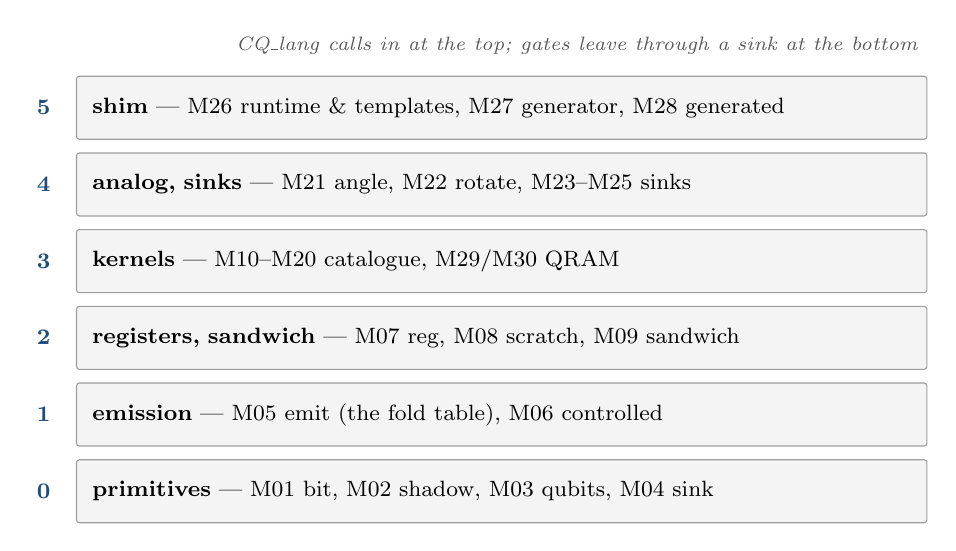
\begin{tikzpicture}[
  font=\footnotesize,
  layer/.style={draw=cqrule, fill=cqbg, rounded corners=1pt,
                minimum height=8mm, text width=104mm, align=left, inner sep=2mm},
  tag/.style={font=\footnotesize\bfseries\color{cqaccent}, anchor=east}]
  \node[layer] (l5) {\textbf{shim} --- M26 runtime \& templates, M27 generator, M28 generated};
  \node[layer, below=1.6mm of l5] (l4) {\textbf{analog, sinks} --- M21 angle, M22 rotate, M23--M25 sinks};
  \node[layer, below=1.6mm of l4] (l3) {\textbf{kernels} --- M10--M20 catalogue, M29/M30 QRAM};
  \node[layer, below=1.6mm of l3] (l2) {\textbf{registers, sandwich} --- M07 reg, M08 scratch, M09 sandwich};
  \node[layer, below=1.6mm of l2] (l1) {\textbf{emission} --- M05 emit (the fold table), M06 controlled};
  \node[layer, below=1.6mm of l1] (l0) {\textbf{primitives} --- M01 bit, M02 shadow, M03 qubits, M04 sink};
  \foreach \n/\t in {l5/5, l4/4, l3/3, l2/2, l1/1, l0/0}
    \node[tag] at ([xshift=-2mm]\n.west) {\t};
  \node[font=\scriptsize\itshape\color{cqsoft}, above=1.5mm of l5.north east, anchor=south east]
    {CQ\_lang calls in at the top; gates leave through a sink at the bottom};
\end{tikzpicture}
\caption*{\small\textbf{The module map.} Layers 0--4 are complete; Layer 5
carries the frozen \texttt{cqrt\_*} ABI. A structural figure --- it encodes the
design, not a measurement.}
\end{figure}

\vspace{4pt}

\subsection*{The steps}

\noindent\small
Sourced from commit subjects; the \textsc{tests} column reproduces the count
each commit recorded for itself at landing, and is therefore a figure at
\emph{that} SHA, not a running total. Decisions are named, never restated.

\vspace{4pt}
\begin{longtable}{@{}p{15mm}p{17mm}p{72mm}p{24mm}@{}}
\toprule
\textsc{step} & \textsc{landed} & \textsc{what} & \textsc{tests}\\
\midrule
\endhead
0     & 2026-08-14 & Bennett.jl and CQ\_lang references pinned on disk; the PRD's internal contradictions resolved & ---\\
1     & 2026-08-14 & Build skeleton, hand-rolled test harness, the 300-line guard & ---\\
2     & 2026-08-14 & \textbf{M01} \texttt{bit.h} --- the tri-valued bit (\textbf{I1}) & ---\\
3     & 2026-08-14 & \textbf{M02} shadow --- the per-qubit \{value, unknown\} table & ---\\
4     & 2026-08-14 & \textbf{M03} qubits, and the shared death-test harness & ---\\
5     & 2026-08-14 & \textbf{M04} sink vtable and the recording mock sink & ---\\
6     & 2026-08-14 & \textbf{M05} emit --- the §3 fold table, the critical path & 159\\
7     & 2026-08-15 & \textbf{M07} reg --- the handle table, and the D7 aliasing split & 46\\
8     & 2026-08-15 & \textbf{M08} scratch + \textbf{M09} sandwich --- the \textbf{I6} driver & 67\\
9     & 2026-08-15 & \textbf{M23} printf sink, \textbf{M24} counting sink & 69\\
10--11 & 2026-08-15 & K1--K5 and the shared Phase-B kernel gate & 87\\
12--13 & 2026-08-16 & K6/K7 add--sub; K9's ten compare predicates & 98\\
14--16 & 2026-08-16 & The barrel shifter, K8's Cuccaro accumulator, K11 \texttt{mul} & 130\\
17--19 & 2026-08-20 & K12 \texttt{divrem}, \textbf{M21} angle, the first rotation & 175\\
20    & 2026-08-20 & \textbf{M06} controlled --- the whole catalogue, no kernel touched & 195\\
21    & 2026-08-21 & The uncompute axis: risk \textbf{R6} had no detector, and now does & 198\\
22--26 & 2026-08-28 & The shim, the QEC sink, and the trace annotations & 310\\
25    & 2026-08-29 & \textbf{L7} Grover --- three claims in three places, three modes & 314\\
\midrule
\multicolumn{4}{@{}l@{}}{\textit{Since, on the same trunk:}}\\
---   & 2026-08-29 & A golden's operand mask made a per-file claim that is read back & 315\\
---   & 2026-09-02 & The free-time residue is read, never printed & 317\\
---   & 2026-09-02 & \textbf{Plan §7: all five finish-line conditions MET}, measured & 317\\
---   & 2026-09-02 & \texttt{tape} in scope as v1.1 (\textbf{D23}) & 325\\
---   & 2026-09-02 & \textbf{QRAM} in scope as v1.2 (\textbf{D24}) --- K13/K14, M29/M30 & 325\\
\bottomrule
\end{longtable}
\normalsize

\vspace{2pt}
\noindent The shape of it: six weeks, Layers 0--4 complete, the five
finish-line conditions met on 2026-09-02, and scope since then widening
deliberately --- \texttt{tape} as v1.1, QRAM as v1.2 --- rather than the
catalogue deepening.

\subsection*{What the catalogue costs}

\noindent The Toffoli count is the figure that matters, because it is what
fault tolerance charges for: measured through the QEC library at $d=3$, one
logical \texttt{CX} is 1{,}830 physical gates and one \texttt{CCX} is
562{,}564 (\textbf{D20}). Only \texttt{xor} is Toffoli-free at every width;
\texttt{and} and \texttt{or} cost exactly $W$, and everything carrying a carry
chain costs more.

\begin{figure}[H]
\centering
\begin{tikzpicture}
\begin{loglogaxis}[
  width=0.92\linewidth, height=70mm,
  xlabel={register width $W$}, ylabel={Toffoli count (forward)},
  xtick={1,2,4,8,16,32,64,128}, xticklabels={1,2,4,8,16,32,64,128},
  log basis x=2, grid=both, grid style={cqrule!30},
  legend pos=north west, legend style={font=\scriptsize, draw=cqrule, fill=white},
  label style={font=\footnotesize}, tick label style={font=\scriptsize},
  every axis plot/.append style={mark size=1.3pt, thick}]
  \addplot table[x=W, y=udiv]  {data/toffoli.dat}; \addlegendentry{\texttt{udiv} (K12)}
  \addplot table[x=W, y=sdiv]  {data/toffoli.dat}; \addlegendentry{\texttt{sdiv}}
  \addplot table[x=W, y=mul]   {data/toffoli.dat}; \addlegendentry{\texttt{mul} (K11)}
  \addplot table[x=W, y=add]   {data/toffoli.dat}; \addlegendentry{\texttt{add} (K6)}
  \addplot table[x=W, y=ult]   {data/toffoli.dat}; \addlegendentry{\texttt{ult} (K9)}
  \addplot table[x=W, y=mux]   {data/toffoli.dat}; \addlegendentry{\texttt{mux} (K10)}
\end{loglogaxis}
\end{tikzpicture}
\caption*{\small\textbf{Quadratic and linear, two decades apart.} \texttt{divrem}
and \texttt{mul} are quadratic in $W$; \texttt{add}, \texttt{ult} and
\texttt{mux} are linear. The gap is why \textbf{D20} bounds what is inspectable
through the QEC sink to Toffoli-\emph{free} regions at small width.}
\datasource{\texttt{docs/labreport/data/toffoli.dat}, pivoted from
\texttt{tests/goldens/*.counts} --- the L4 pins themselves, at the all-quantum
operand mask. A count is a function of $(W,\text{mask})$.}
\end{figure}


%% ==========================================================================
%% ENTRIES — append below, never reorder, never edit an existing line.
%% ==========================================================================
%% labreport entry 1 — 2026-09-10
%% labreport-to: 3464bf5
%%
%% APPEND-ONLY. Once this entry is committed it is never edited: a later
%% correction is a NEW entry carrying \supersedes{1}{field}.

\entry{1}{2026-09-10}{D20's scratch figure, and this report}

\begin{generated}
  \gitem{Range}{\texttt{a78c12b..3464bf5}}
  \gitem{Tree}{\emph{dirty at capture} --- 12 path(s) uncommitted}
  \gitem{Tests}{Release \textbf{356/356}, Debug \textbf{357/359} --- the two
         being \texttt{l6\_cqlang\_fixtures} and \texttt{l7\_grover\_cqlang}, both
         red from upstream drift (\bead{w9i}, \bead{2tm})}
  \gitem{LOC}{OK --- 203 file(s), limit 300, largest 297 (\texttt{tests/test\_kernel\_add.c})}
  \gitem{Commits}{\begin{commitlist}
    \item \texttt{3464bf5} \bead{fxz}: PRD §15 D25 --- a kernel whose scratch
          region does not fit the D2 ceiling \emph{(the prior session's work,
          landed here)}
  \end{commitlist}}
  \gitem{Beads closed}{\bead{j75} D20 cites 79 scratch qubits for K12 at $W=8$;
         \texttt{cq\_divrem\_region} says 543}
  \gitem{Beads filed}{\bead{y1i} D20 says \texttt{cq\_kernel\_xor} at $W=4$ is
         4 CX; the L4 golden says 8 \quad \bead{2tm} L7's
         \texttt{grover.cq.c} calls the retired two-argument \texttt{cq\_phi}}
  \gitem{Beads updated}{\bead{w9i} re-measured: 3 affected fixtures $\to$ 23}
\end{generated}

\field{The ask}
Implement \bead{j75}; then design and build a lab report --- an append-only,
human-readable \LaTeX{} document carrying one entry per session --- and put the
rule that maintains it into \texttt{CLAUDE.md}.

\field{What landed}
\textbf{PRD~§15~D20's scratch-qubit citation is corrected} and carries a dated
note saying what the old figure actually was, so the number cannot quietly
travel again. \textbf{This document exists}: master file, masthead, a
reconstructed prologue covering Steps 0--26, two generators
(\texttt{tools/labreport/new\_entry.py} for an entry's extracted header,
\texttt{gen\_data.py} for figure data), a \texttt{make labreport} target that
probes for \texttt{pdflatex} rather than assuming it, and the session rule in
\texttt{CLAUDE.md}. The PDF is gitignored --- the \texttt{.tex} is the artefact.

\field{Measured}
D20 read \emph{``K12's \texttt{divrem} at $W=8$ alone takes $W^2+2W-1 = 79$
scratch qubits before operands''}. That formula is K12's \emph{remainder tape},
one component of the region --- \texttt{divrem\_u.h} says so in its own header
comment. The region is $8W^2+4W-1$, and the bound a bounded device actually has
to meet is higher still: the \emph{peak}, because \texttt{dst}'s lanes are
materialised by the copyout while the whole region is still live (\textbf{D25}(a)).

\begin{figures}
\fig{543}{\texttt{cq\_divrem\_region(8,\,1)}, probe linked against the archive}{Release}
\fig{551}{\texttt{cq\_kd\_peak}, high-water mark during the call}{Release}
\fig{131{,}583}{\texttt{cq\_divrem\_region(128,\,1)} --- K12 at i128}{Release}
\fig{79}{\emph{the retired figure} --- K12's remainder tape, not its region}{---}
\end{figures}

\noindent The error ran in the direction that \emph{weakened D20's own
argument}: the row is arguing that the pool ceiling is hard against
\texttt{qec\_n\_logical} values the shipped configs cap at 7, and 543 makes that
case seven times harder than 79 did. A citation error that flatters its own
argument is the one nobody re-derives --- which is why the correction is worth
more than the number.

\begin{figure}[H]
\centering
\begin{tikzpicture}
\begin{axis}[
  width=0.92\linewidth, height=66mm,
  xlabel={register width $W$}, ylabel={scratch qubits},
  grid=both, grid style={cqrule!30}, xmin=1, xmax=33,
  legend pos=north west, legend style={font=\scriptsize, draw=cqrule, fill=white},
  label style={font=\footnotesize}, tick label style={font=\scriptsize},
  every axis plot/.append style={mark size=1.2pt, thick}]
  \addplot table[x=W, y=divpeak]   {data/scratch.dat}; \addlegendentry{K12 \texttt{udiv} --- peak}
  \addplot table[x=W, y=divregion] {data/scratch.dat}; \addlegendentry{K12 \texttt{udiv} --- region}
  \addplot table[x=W, y=mulpeak]   {data/scratch.dat}; \addlegendentry{K11 \texttt{mul} --- peak}
  \draw[cqrule, dashed] (axis cs:8,0) -- (axis cs:8,551);
  \node[font=\scriptsize\color{cqsoft}, anchor=west] at (axis cs:9,700)
    {$W=8$:\ \ peak 551,\ region 543};
\end{axis}
\end{tikzpicture}
\caption*{\small\textbf{Region is not peak, and neither is the tape.} The two
K12 curves are close enough to look interchangeable and are not: the copyout
runs while the region is live, so a device holding exactly the region does not
run the kernel. The retired figure, 79, is off this chart entirely at $W=8$.}
\datasource{\texttt{docs/labreport/data/scratch.dat}, written by a probe
\emph{run} against \texttt{build-release/libcqops.a} --- not from a formula.}
\end{figure}

\noindent\textbf{And the apparatus found a second one immediately.} Plotting the
catalogue put the pinned counts next to the prose ones, and the \emph{same row}
of D20 says \texttt{cq\_kernel\_xor} at $W=4$ is 4~CX where
\texttt{tests/goldens/bitwise.counts} pins 8 --- K1 is
\texttt{dst\,\^{}=\,a\,\^{}\,b}, one CX per source per lane, so the count is
$2W$. Filed as \bead{y1i} rather than fixed in passing, for the reason
\bead{j75} itself records. Its direction is the \emph{opposite} of
\bead{j75}'s and D20's conclusion survives either way --- the row argues the cost
is small enough to draw, and $2\times$ is still far inside the drawer's limits.
It is the case for generating figure data rather than typing it, made on the
first day the generator existed.

\field{Decided}
\textbf{PRD~§15~D20} is amended in its citation only; it is not re-resolved and
takes no new D-number. \textbf{D25} and \textbf{D9}(a), which the corrected
sentence now points at, are untouched. The report's own rule goes into
\texttt{CLAUDE.md} under \emph{Session Completion}.

\field{Not taken}
\textbf{Backfilled per-session entries for Steps 0--26} --- the prologue is one
table and is flagged as a reading of the record rather than an account of it;
inventing 27 retrospective ``sessions'' would put prose in the document that
nobody lived. \textbf{A shared figures directory} --- rejected because an
\texttt{\textbackslash input} shared between entries silently changes an old
entry when it is updated, and nobody diffs a rendered PDF; figures live inside
the entry that uses them. \textbf{Committing the PDF} --- the user's call, and
the right one. \textbf{A 2--5 page quota per entry} --- proposed and dropped: a
quota manufactures narrative, and inflated significance in a document future
sessions mine is worse than no document.

\field{Verified}
\bead{j75} itself is docs-only. But the session also \emph{landed} the prior
session's uncommitted D25 work, so the full gate was run rather than assumed:
\textbf{Debug 357/359, Release 356/356} (the latter excluding the two entries
below). \texttt{tools/check\_loc.sh} passes at 203 files, and this document
compiles under \texttt{pdflatex}. The scratch figures come from two probes built
against \texttt{build-release/libcqops.a}; \texttt{test\_kernel\_divrem} case~6,
where the region and the peak are both pinned, is green.

\medskip
\noindent\textbf{Two entries are RED and are not ours.}
\texttt{l6\_cqlang\_fixtures} and \texttt{l7\_grover\_cqlang} both fail against
CQ\_lang \texttt{5a26204}; the last measurement in this repo was against
\texttt{893b769}, and \textbf{this repo neither pins nor can build CQ\_lang}, so
these two track a moving target by design. L6: 100 OK, 201 deferred,
\textbf{23 build failures, all on one undefined symbol} ---
\texttt{cqrt\_ry\_i32\_controlled}, emitted by CQ\_lang and declared by nothing we
vendor, which is \bead{w9i} exactly (filed when it hit 3 fixtures). \texttt{nm}
confirms our archive defines the \texttt{\_inv} sibling and not this one, so it
was never ours to define; the OK count in fact \emph{rose}, 71 to 100, far clear
of the floor of 43. L7 is a different cause, newly filed as \bead{2tm}:
\texttt{cq\_phi} has become a register-free \texttt{void cq\_phi(double)} upstream
and our fixture still passes it two arguments. \textbf{Neither is caused by
anything committed here} --- the whole unit, death and shim surface is green in
both configurations at the same tree.

\field{Left open}
24 beads open, none claimed; \bead{y1i} and \bead{2tm} filed, \bead{w9i}
re-measured. Six are now citation/staleness
bugs of the same family as \bead{j75} --- \bead{y1i}, \bead{0a7}, \bead{18f},
\bead{dtb}, \bead{eh9}, \bead{wf8} --- and are the obvious next batch, being
cheap and mutually independent --- and two of the six were found by an
instrument rather than by reading.

% labreport entry 2 — 2026-09-10
% labreport-to: 0389705
%%
%% APPEND-ONLY. Once this entry is committed it is never edited: a later
% correction is a NEW entry carrying \supersedes{2}{field}.

\entry{2}{2026-09-10}{the frozen ABI re-vendored at 182}

\begin{generated}
  \gitem{Range}{\texttt{3464bf5..0389705}}
  \gitem{Tree}{\emph{dirty at capture} --- 19 path(s) uncommitted}
  \gitem{Tests}{Release \textbf{358}, Debug \textbf{359} registered
         (\texttt{ctest -N}); pass counts are in \emph{Verified}}
  \gitem{LOC}{OK — 203 file(s), limit 300, largest 297 (tests/test\_kernel\_add.c)}
  \gitem{Commits}{\begin{commitlist}
    \item \texttt{0389705} bd j75: D20's scratch figure was the remainder tape,
          not the region; and the lab report \emph{(entry 1's work, committed
          after it was written --- this entry's own work is uncommitted at
          capture, so the extracted Beads rows below describe that commit and
          not this session)}
  \end{commitlist}}
  \gitem{Beads closed}{\bead{fxz} M18: mul at i128 needs 16,640 scratch qubits — document the loud failure at the D2 pool ceiling, \bead{j75} PRD §15 D20 cites 79 scratch qubits for K12 at W=8; cq\_divrem\_region says 543}
  \gitem{Beads filed}{\bead{cxp} [bug] PRD §12's listing and §15 D22 carry the retired two-argument cq\_phi, which is now a compile error upstream, \bead{2tm} L7: tools/l7/grover.cq.c calls the retired two-argument cq\_phi and no longer compiles, \bead{y1i} PRD §15 D20 says cq\_kernel\_xor at W=4 is 4 CX; the L4 golden says 8, \bead{j75} PRD §15 D20 cites 79 scratch qubits for K12 at W=8; cq\_divrem\_region says 543}
  \gitem{Diff}{\texttt{14 files changed, 1929 insertions(+), 2 deletions(-)}}
\end{generated}

%% ---- Hand-written below. Omit any field the session did not earn; a
%% ---- one-bead session is a paragraph, not a page. Fields 1, 2 and 6 are
%% ---- the ones that are never omitted.

\field{The ask}
Take \bead{w9i} --- the last red gate not caused by anything in this repo ---
now that CQ\_lang has committed the ABI widening it was filed against. Confirm
first that the previous session's uncommitted work passes its gate, which had
never been run to completion.

\field{What landed}
\textbf{The frozen \texttt{cqrt\_*} ABI is re-vendored at CQ\_lang
\texttt{170ede1}, 173 $\to$ 182 declarations}, and \textbf{L6 is green for the
first time since \bead{w9i} was filed} --- all 23 build failures gone, none
replaced. The nine new symbols are one family, \texttt{cqrt\_ry\_<W>\_controlled},
which \textbf{PRD~§15~D16} splits 5 integer \emph{implemented}
(\texttt{shim/cq\_runtime\_gate.c}, the \texttt{\_controlled\_inv} body without
its \texttt{-angle}) and 4 fp \emph{deferred}
(\texttt{shim/cq\_runtime\_v2.c}). Six prose sites that asserted
\emph{``there is no plain \texttt{cqrt\_ry\_<W>\_controlled} at any width''} are
corrected in place, each carrying what it used to say.

\field{Measured}
\begin{figures}
\fig{182}{comment-stripped identifier extraction over both headers; \textbf{nine pure insertions, no existing signature moved}}{---}
\fig{0}{\texttt{diff} of normalised declarations, excluding the nine --- signature drift}{---}
\fig{123/201/0}{\texttt{l6.json} OK / DEFERRED / \textbf{BUILD\_FAIL}, was 100/201/23}{Release}
\fig{180}{\texttt{nm -g} on \texttt{libcqops.a}, defined \texttt{cqrt\_*} --- 182 less the two \texttt{cqrt\_h*}}{Release}
\fig{39}{\texttt{cqrt\_ry\_i32\_controlled} calls in CQ\_lang's e2e goldens, over 23 fixtures}{---}
\end{figures}

\noindent\textbf{\texttt{opcode\_table.yaml} did not move} --- sha256
\texttt{6245117d\dots a3e82426} at both revisions --- so the 2{,}479
\texttt{cq\_template\_*} grid is untouched and \textbf{nothing under
\texttt{third\_party/} was written}. \bead{w9i}'s recipe says to re-pin
\texttt{third\_party/cq\_lang/COMMIT} as well; that would have been wrong, since
the artefact it pins is byte-identical and re-pinning would claim a re-vendor
that did not happen.

\medskip
\noindent\textbf{The population pins went red on purpose in FIVE places and the
bead names four.} The fifth is
\texttt{cmake/CqopsLinkWitness.cmake}'s \emph{generated}
\texttt{\textbackslash{}\_Static\_assert(CQ\_LINK\_C\_ROWS == 171)}, which fails at
\emph{build} time rather than test time and whose message names neither a test
nor the count's owner.

\medskip
\noindent\textbf{And a shipped comment's corpus claim went false in the same
motion.} \texttt{cq\_runtime\_gate.c} read \emph{``measured demand today: zero
controlled rotations of any kind''}. Re-measured: \textbf{39}, all
\texttt{ry\_i32}, across the same 23 fixtures. They all \emph{run}, because their
four distinct angles ($\pm0.6$, $0.7$, $0.9$~rad) are far from the
$\pi$-lattice and take §7's general row --- so \textbf{D11's refusal surface is
still reached by the corpus zero times}, which is the same position as before
with one fewer assumption in it. PRD~§9~row~B also holds on the new traffic:
control $\neq$ target in all 39.

\field{Decided}
\textbf{PRD~§15~D16} gains its second worked example and it runs the
\emph{opposite} way from the first: where \texttt{cqrt\_qram\_alloc\_f32} shows a
family overriding an fp token, \texttt{cqrt\_ry\_f32\_controlled} shows an fp token
deferring a family that is otherwise in scope. D16 is amended, not re-resolved,
and takes no new D-number. \textbf{PRD~§2.1}'s controlled row and
\textbf{§15~D11}'s demand figure are corrected.

\field{Not taken}
\textbf{Implementing all nine widths uniformly} --- asked for, and declined on a
fact that was not on the table when it was asked: \texttt{cqrt\_alloc\_f<W>} is
itself an abort, so \emph{no fp rail handle can exist at runtime in v1}. An
implemented body would resolve its handle through M07 and take M07's
\emph{generic} error instead of \texttt{cq\_shim\_unsupported}'s named one ---
worse diagnostics on a path nothing can reach, a forward implemented where its
own \texttt{\_inv} is not, and the only implemented fp rotation of any kind. The
abort's reason string is \texttt{"fp is v2"}, which \emph{is} the capability
claim, and is what those four bodies become when fp lands.
\textbf{Leaving L6 red by design} --- weighed: the blast radius had gone
3~$\to$~10~$\to$~23 fixtures in eight days, so waiting was not free either.
\textbf{Re-running L6 in Debug} --- $\sim$25~min under sanitizers, and the claim
it makes is a LINK claim that does not vary by configuration.

\field{Verified}
Rule 17, literally. \texttt{make lint} OK (203 files, largest 297).
\textbf{Release 357/357 and Debug 358/358} with \texttt{l6\_cqlang\_fixtures}
excluded, both after the change; \texttt{l7\_grover\_cqlang} is inside those
counts and passed. \textbf{L6 was then run once, clean, in Release only}:
\textbf{passed}, 563~s, 324 fixtures, \textbf{0 build failures}. The
\texttt{--gate} clause is what had been failing --- a \texttt{BUILD\_FAIL} is
neither OK nor DEFERRED --- and the floor (\texttt{CQOPS\_L6\_MIN\_OK}=43) was
never in play.

\medskip
\noindent The re-vendored copy was verified the way its own banner prescribes:
compiled \emph{together with} upstream's header, zero \texttt{conflicting types},
with a one-parameter-widened negative control producing exactly one. Residue over
the 123 completing fixtures: \textbf{992 qubits unproven over 58 unproven frees,
0 convicted, 0 dirty}, 20 fixtures reporting --- unchanged in kind.

\medskip
\noindent\textbf{Two new cases, because the forward twin is a comparison the
tree could not make before.}
\texttt{ry\_controlled\_inv\_is\_ry\_controlled\_at\_a\_negated\_angle} pins the
promoted four-gate general row as an \emph{ordered, bitwise} stream comparison
--- a transposed $R(\pm\theta/2)$ or a forgotten negation moves it and moves no
count. \texttt{a\_controlled\_ry\_taints\_its\_target\_and\_a\_controlled\_rz\_does\_not}
is a claim about the \emph{record} layer:
\texttt{cq\_shim\_record.c} marks \texttt{first\_rot} for the non-diagonal Ry rows
\emph{by naming them}, so a row added to the effect table but not to that list
would leave a controlled forward Ry looking diagonal to D15's certificate and a
rail it rotated could be released CLEAN.

\field{Left open}
\bead{w9i} is ready to close. \bead{cxp} and \bead{2tm} landed in the previous
session and their gate is now confirmed. The staleness family --- \bead{y1i},
\bead{0a7}, \bead{18f}, \bead{dtb}, \bead{eh9}, \bead{wf8} --- is untouched and
remains the obvious next batch; \bead{0a7} is \emph{worse} for this session's
work, since the PRD gained roughly thirty lines above the K-doc citation targets.
\textbf{The standing hazard is unchanged}: this repo neither pins nor can build
CQ\_lang, so L6 tracks a moving target by design and today's green is a
measurement, not a property.

% labreport entry 3 — 2026-09-10
% labreport-to: 961905f
%%
%% APPEND-ONLY. Once this entry is committed it is never edited: a later
% correction is a NEW entry carrying \supersedes{3}{field}.

\entry{3}{2026-09-10}{the stale-claims batch: eight beads sorted three ways}

\begin{generated}
  \gitem{Range}{\texttt{0389705..961905f}}
  \gitem{Tree}{\emph{dirty at capture} --- 27 path(s) uncommitted}
  \gitem{Tests}{Release \textbf{358}, Debug \textbf{359} (\texttt{ctest -N})}
  \gitem{LOC}{OK — 203 file(s), limit 300, largest 297 (tests/test\_kernel\_add.c)}
  \gitem{Commits}{\begin{commitlist}
    \item \texttt{961905f} bd w9i: re-vendor the frozen cqrt\_* ABI at CQ\_lang 170ede1 (173->182); cqrt\_ry\_<W>\_controlled 5 int implemented / 4 fp deferred per D16; L6 100->123 OK, 0 BUILD\_FAIL \emph{(entry 2's work, committed after it was
          written --- this session's own work is uncommitted at capture, so
          the Range and Diff rows describe THAT commit, and the Beads rows
          below are every bead closed or filed anywhere on 2026-09-10, which
          is all three of today's sessions and not this one)}
  \end{commitlist}}
  \gitem{Beads closed}{\bead{cxp} [bug] PRD §12's listing and §15 D22 carry the retired two-argument cq\_phi, which is now a compile error upstream, \bead{2tm} L7: tools/l7/grover.cq.c calls the retired two-argument cq\_phi and no longer compiles, \bead{w9i} CQ\_lang's dirty tree widens the frozen ABI: cqrt\_ry\_<W>\_controlled is emitted by three untracked fixtures and declared by nothing we vendor, \bead{1ti} The corpus 'moved four times on 2026-08-22' is asserted in four places; D15 section 0 enumerates two transitions per series, \bead{fxz} M18: mul at i128 needs 16,640 scratch qubits — document the loud failure at the D2 pool ceiling, \bead{o63} K01/K02 section 5 delta-2 upstream comparisons are fold\_constants=false figures; Bennett folds BY DEFAULT, \bead{y1i} PRD §15 D20 says cq\_kernel\_xor at W=4 is 4 CX; the L4 golden says 8, \bead{j75} PRD §15 D20 cites 79 scratch qubits for K12 at W=8; cq\_divrem\_region says 543, \bead{dtb} check\_loc.sh scans tools/ but its own header and three documents say four roots, \bead{18f} K06.md and K07.md still say UNVERIFIED-BY-EXECUTION; Step 12 measured them and only CLAUDE.md records it, \bead{wf8} K05.md carries two stale self-assessments that are Rule 16 traps, \bead{eh9} PRD section 13 increment 2 asks only for L1/L2/L5 on K1-K5; plan section 4 Phase B applies L1-L4 at every kernel step, \bead{0a7} K01-K03 line-number citations into PRD-v1.md and IMPLEMENTATION\_PLAN.md are stale by 95-183 lines}
  \gitem{Beads filed}{\bead{cxp} [bug] PRD §12's listing and §15 D22 carry the retired two-argument cq\_phi, which is now a compile error upstream, \bead{2tm} L7: tools/l7/grover.cq.c calls the retired two-argument cq\_phi and no longer compiles, \bead{j5v} check\_cites.sh's target set stops at the four planning docs: 20 living-target line cites INTO K-docs and BASELINES.md remain bare (src/, tests/, plan, K12->K09), \bead{16q} D15's carve-out witnesses have moved out from under it at CQ\_lang HEAD: the ckd.18 shape counts ZERO and slice\_loop\_break* is five -> four, \bead{aei} tests/test\_kernel\_cast.c:83-85 says the small-width sweep is exhaustive; every width has been a 32-case sample since 2026-08-21, \bead{iwn} tests/test\_kernel\_add.c is at 297/300 with no recorded seam beyond the \_upstream.inc split, \bead{65q} D20's per-gate physical costs (CX 1,830 / CCX 562,564 at d=3) are pinned by no test and by no QEC revision, \bead{wgi} tools/l6/l6\_run.py is at 281/300 and past plan §3 Layer 6's recorded split trigger (240), \bead{y1i} PRD §15 D20 says cq\_kernel\_xor at W=4 is 4 CX; the L4 golden says 8, \bead{j75} PRD §15 D20 cites 79 scratch qubits for K12 at W=8; cq\_divrem\_region says 543, \bead{bz8} K06/K07 follow-ups from bd 18f: evaluated tables stop at W=64 (goldens run to 128); 'does CQ\_lang ever pass a constant register to cq\_template\_add\_*' is now measurable off L6, \bead{bpw} K05 §5 item 5 says a cast with T == F should be refused; src/kernels/cast.c:15-20 accepts it as an identity copy -- decide which, \bead{a9e} check\_loc.sh's printed file COUNT is box-local: it walks the filesystem, not the git index, and tools/qtg/ is gitignored}
  \gitem{Diff}{\texttt{24 files changed, 805 insertions(+), 115 deletions(-)}}
\end{generated}

%% ---- Hand-written below. Omit any field the session did not earn; a
%% ---- one-bead session is a paragraph, not a page. Fields 1, 2 and 6 are
%% ---- the ones that are never omitted.

\field{The ask}
Eight beads of one kind: a claim in a document or a shipped comment that was
true when it was written and is false now, or a citation that has rotted. The
method is \bead{cxp}'s three-way sorting --- \emph{protected source intent},
\emph{live present-tense claim now false}, \emph{dated measurement} --- and the
\emph{sorting} is the deliverable, not the edit count: a batch that changes
eight numbers and sorts them wrongly is worse than one that changes three and
records why the other five stay. Re-measure every figure against the artefact,
never against a remembered formula. Serialize the PRD editors; take \bead{0a7}
last and alone.

\field{What landed}
\textbf{Eight beads closed, and every site now carries the category it was
sorted into rather than only its new value.}

\begin{itemize}[leftmargin=1.5em,itemsep=2pt,topsep=4pt,parsep=0pt]
\item \bead{o63} --- K01/K02/K03 §5's \emph{deltas from upstream}: all three
      sites \textbf{category 2}, corrected in place carrying the old figure
      qualified as a \texttt{fold\_constants=false} number. K02's advertised win
      is \emph{retracted} --- see \emph{Measured}.
\item \bead{1ti} --- the ``corpus moved four times on 2026-08-22'' claim, in five
      places, resolved as the bead's own reading (b). §0's blanket sentence is
      \textbf{category 2}; §0's enumeration is \textbf{category 3}, verbatim
      under a dated amendment carrying the per-revision table. The pin itself was
      also wrong --- see \emph{Decided}.
\item \bead{y1i} --- \textbf{PRD~§15~D20}(2)'s parenthetical: \textbf{category
      3}, verbatim with a dated amendment, the shape \bead{j75} established one
      session earlier; the neighbouring \texttt{add} figure re-measured
      \emph{right}.
\item \bead{18f} --- K06.md and K07.md: the \textsc{unverified-by-execution}
      subsections are \textbf{category 3} and stay verbatim under a dated banner
      in K09's Step-13 shape, over four \textbf{category 2} corrections. Pure
      insertions, zero deletions.
\item \bead{wf8} --- K05.md, 15 sites: the two the bead named plus 13 of the same
      class in the same file. \textsc{unverified-by-execution} is \textbf{category
      1} here --- \texttt{which julia} is still empty, so the label is true and it
      was its \emph{explanation} that was false.
\item \bead{eh9} --- \textbf{PRD~§13}'s increment 2 against \textbf{plan~§4}'s
      Phase~B gate: a head note plus rows 2 and 7 corrected under strikethrough.
      Rows 3--6 were true as written and were left alone.
\item \bead{dtb} --- \texttt{tools/check\_loc.sh} has scanned \emph{five} roots
      since Step~1 (\texttt{0cc70e3}) while its header, \textbf{CLAUDE.md
      Rule~12} and \textbf{plan~§2.3} all said four. All \textbf{category 2}; the
      ``harmless today'' that excused it is dead.
\item \bead{0a7} --- every citation from a living document into a living document
      now carries a section, a quoted phrase and a line number \emph{pinned to a
      commit}, and \texttt{tools/check\_cites.sh} is in \texttt{make lint} and the
      CMake \texttt{lint} target so the bare form cannot come back. The form, its
      scope and the guard's timing are the maintainer's --- recorded in the bead
      and in the guard's own header.
\end{itemize}

\noindent\textbf{No compiled line changed.} The eight source files in the diff
are comment-only; the only executable additions are the guard and the two lines
that wire it in.

\field{Measured}
\begin{figures}
\fig{3 of 4}{\texttt{git ls-tree} plus a \texttt{cqrt\_free(} line count over
     CQ\_lang's history for 2026-08-22: golden-set moves against commits touching
     \texttt{tests/e2e}}{--- (read-only)}
\fig{240 / 51{,}698}{the same at \texttt{397c67c}; \textbf{D15~§0's pin says
     241 / 51{,}705} --- \texttt{7385c4d}'s pair}{--- (read-only)}
\fig{8 CX}{\texttt{tests/goldens/bitwise.counts}, \texttt{xor} at $W=4$, forward
     and \texttt{\_unc}; D20 says 4}{Release goldens, all-quantum}
\fig{8 CNOT + 8 NOT}{a hand-walk of \texttt{\_fold\_constants} at Bennett's
     \emph{default} for \texttt{x \^{} 0x0f}, $W=8$ --- a \textbf{reading},
     \textbf{Julia absent}}{---}
\fig{16/16, 16/16, 20/20}{\texttt{add.counts} against K06's and K07's closed
     forms (eight widths $\times$ \{forward, \texttt{\_unc}\}), and
     \texttt{cast.counts} against K05~§3e}{Release goldens}
\fig{203 = 60+1+102+24+16}{\texttt{tools/check\_loc.sh} per root; the fifth is
     \texttt{tools/}, largest \texttt{l6\_run.py} at 281}{---}
\fig{101 $\to$ 0}{\texttt{tools/check\_cites.sh}: bare living-target line cites
     over 296 files, before conversion and after}{---}
\fig{142}{pins written --- \textbf{130} mechanically (phrase unique in the tree
     \emph{and} inside the pinned range at the SHA), \textbf{12} by hand as
     extractor artefacts}{---}
\fig{53 / 6}{section labels machine-checked against the heading map @
     \texttt{961905f} / how many were wrong}{---}
\end{figures}

\noindent Two survey figures that decided the \bead{0a7} form rather than
measuring its result: \textbf{277 of 277} pinned \texttt{.jl} citations into
\texttt{third\_party/bennett/} resolve, against \textbf{2 of 29} plan citations
and \textbf{0 of 53} PRD citations; and the guard flagged \textbf{7 of 18}
crafted provocation cases, exactly the right seven.

\medskip
\noindent\textbf{The K02 win does not exist at Bennett's default, and that
retraction is the whole of \bead{o63}.} K02~§5 advertised \emph{``Bennett pays
4~NOT + 8~Toffoli, libcqops pays zero Toffoli''} for \texttt{x \& 0x0f}; walked
at default options the pass emits \textbf{4 CNOT + 4 NOT + 0 Toffoli}, and
zero-Toffoli against zero-Toffoli is not a delta. All three examples give one
uniform result --- upstream's folded cost exceeds ours by exactly
$p = \mathrm{popcount}(k)$ NOTs, the end-of-circuit re-materialisation --- and
\texttt{\_fold\_constants} deletes gates \emph{without} renumbering or releasing
wires, so upstream still stands up $2W$ non-input wires where we allocate $p$.
\textbf{The headline formulas and the L4 goldens are unaffected}: they are pinned
at the all-quantum mask, where the fold pass provably does nothing.

\medskip
\noindent\textbf{And one document was right about its symptom and wrong about
its cause.} K05 explained its stale cast grid by ``the live tree may be ahead of
the PRD''. Re-measured: \texttt{opcode\_table.yaml}'s sha256 is byte-identical to
CQ\_lang's live copy at \texttt{170ede1}, last touched \texttt{4d5ba4e}
(2026-07-15) --- the PRD simply lacked i80 then. A correct symptom with a
fabricated cause survives a re-read, because the half a reader checks is true.

\medskip
\noindent\textbf{The review round caught something on seven of the eight beads,
and the recurring shape is ``the anchor half right, the human half wrong''.} A
\emph{silent re-partition} of K05~§6's ``Inferred'' list --- claimed kept, in
fact re-split with one clause deleted unquoted, restored verbatim from
\texttt{HEAD} with dated verdicts hung off each item; a citation outside its
scope in all three \bead{o63} sites; an \texttt{awk} hex-float coercion that read
\texttt{-0x1.921fb54442d18p+0} as 0 and so made every float-born rail look
born-zero, producing a population figure that did not exist; six wrong
\emph{section} labels among \bead{0a7}'s pins, whose line numbers and quoted
phrases were all correct; and the guard's own worked example citing a line its
phrase is not on --- a pin failing its own check, inside the message printed on
every failure. Two shell traps came out of it: zsh applies the \texttt{:P}
history modifier inside \texttt{"\$c:FILE"}, so \texttt{git show} answers ``the
text never existed'' rather than failing; and \texttt{git log -{}- FILE} answers
about commits that \emph{touched} a file, not commits where the file merely
\emph{holds} the content --- so ``never there'' and ``never edited'' come back as
the same silence.

\field{Decided}
\bead{0a7}'s three answers are the maintainer's, asked rather than guessed: the
hybrid citation form, its full scope, and the guard now rather than later. They
are recorded in the bead and in \texttt{tools/check\_cites.sh}'s header and are
not restated here. \bead{eh9} was a routine orchestrator call --- \emph{both} of
the two fixes the bead offered, not one. \bead{1ti} resolved as its own reading
(b), and \textbf{PRD~§15~D15~§0} gains a dated amendment: its pin was off by one
commit, and \textbf{D15~§4}'s \texttt{ckd.18} shape identifies the revision the
decision was measured at independently of the corpus counts. D15 is amended in
its figures only --- not re-resolved, and it takes no new D-number.

\field{Not taken}
\textbf{Re-measuring the line numbers and leaving them bare} --- the measured rot
rate puts a re-anchored line out of date again in about three commits, and this
had been tried and had failed four times, K08, K09, K11 and K12 each recording a
cycle. \textbf{Anchor-only, dropping the line} --- loses the literal
reproducibility \texttt{git show <sha>:FILE | sed -n Np} is exactly what buys.
\textbf{Dropping \texttt{tools/} from \texttt{check\_loc.sh}} to make the
documents true --- would un-guard 16 files, one at 281/300; the documents were
corrected instead. \textbf{Reconciling D15~§2's four-way decomposition by running
L6} --- three of its four terms are runtime classifications, so the figure stands
with a dated note saying it was not re-run. \textbf{Re-measuring D20's per-gate
physical cost} --- no QEC revision is pinned here, so the 2026-08-28 trace-driver
numbers were reused \emph{as recorded} and the gap filed as \bead{65q}.
\textbf{Widening PRD~§13's rows 3--5} --- true as written, and editing a true row
to look consistent is the failure this batch was set up to avoid.

\field{Verified}
Rule 17, literally. \texttt{make lint} \textbf{OK} at every step --- 203 files,
limit 300, largest 297 (\texttt{tests/test\_kernel\_add.c}) --- and from
\bead{0a7} onward the same invocation carries the second guard:
\texttt{check\_cites: OK --- 296 file(s) scanned, 0 bare living-target line
citations}, under both \texttt{make lint} and the CMake \texttt{lint} target.
\textbf{The full gate ran three times} --- after the source edits were final,
after the guard landed, and after the review fixes --- and every one of the three
was \textbf{Release 357/357 and Debug 358/358}, with
\texttt{l6\_cqlang\_fixtures} excluded in both, which is the whole difference
between those and the 358 / 359 \emph{registered} in the header above. Single
suites were also run directly against the prebuilt binaries while the evidence
was being gathered: \texttt{test\_kernel\_bitwise} 11/11 and
\texttt{test\_kernel\_shift} 13/13 in \textbf{Release},
\texttt{test\_kernel\_cast} 10/10 and \texttt{test\_kernel\_add} 13/13 --- plus
its two death cases --- in \textbf{both} configurations.

\medskip
\noindent\textbf{L6 was not run, and the reason is what it claims.} It is a LINK
claim, $\sim$9~min in Release and $\sim$25 in Debug, and every source edit here is
a comment. It was green at \texttt{961905f} --- \textbf{123 OK / 201 DEFERRED /
0 BUILD\_FAIL} against CQ\_lang \texttt{170ede1} --- and CQ\_lang's HEAD moved
twice more \emph{during} this session (\texttt{170ede1} $\to$ \texttt{a34cd22}
$\to$ \texttt{8a8f8cf}, 323 $\to$ 332 goldens), so that green already describes a
revision behind the one a re-run would meet.
\textbf{Julia is absent} (\texttt{which julia} empty), so every Bennett-side
figure in \bead{o63}, \bead{18f} and \bead{wf8} is a transcription or a hand-walk
of the pass, and each document says so where it stands.

\field{Left open}
\textbf{Nine beads filed, none claimed.} \bead{j5v} --- 20 living-target line
cites \emph{into} the K-docs and \texttt{BASELINES.md} (from \texttt{src/},
\texttt{tests/}, the plan, and K12 into K09) stay bare, because the guard's
target set stops at the four planning docs; that is the next increment of
\bead{0a7}'s form. \bead{16q} --- \textbf{D15}'s carve-out witnesses have moved
out from under it at CQ\_lang HEAD, where the \texttt{ckd.18} population is now
zero; whether to re-pin the decision at a newer revision is a decision, not a
measurement, and is left to the maintainer. \bead{bpw} --- K05~§5 says a cast
with $T = F$ should be refused where \texttt{src/kernels/cast.c} accepts it as an
identity copy; unreachable from the shipped grid, so it is a call about which
document is right. \bead{65q}, \bead{aei}, \bead{iwn}, \bead{wgi}, \bead{bz8}
and \bead{a9e} are the smaller residue: an unpinned QEC per-gate cost, a false
``exhaustive'' comment, a box-local file count, two files near the 300-line limit
(\texttt{test\_kernel\_add.c} at 297 with no recorded seam, \texttt{l6\_run.py} at
281 and past plan~§3's recorded split trigger of 240), and the K06/K07
follow-ups. \textbf{Nothing is committed}: the working tree carries 26 modified
files (1{,}207 insertions, 190 deletions) plus the new
\texttt{tools/check\_cites.sh}, and the commit awaits approval.

% labreport entry 4 — 2026-09-11
% labreport-to: 2d917b6
%%
%% APPEND-ONLY. Once this entry is committed it is never edited: a later
% correction is a NEW entry carrying \supersedes{4}{field}.

\entry{4}{2026-09-11}{CI wired up, and three Rule-12 splits measured before they were cut}

\begin{generated}
  \gitem{Range}{\texttt{961905f..2d917b6}}
  \gitem{Tests}{Release \textbf{358}, Debug \textbf{359} (\texttt{ctest -N})}
  \gitem{LOC}{OK — 204 file(s), limit 300, largest 294 (tests/test\_unc.c)}
  \gitem{Commits}{\begin{commitlist}
    \item \texttt{2d917b6} bd kju/wgi/iwn/y0f: CI wired up (ubuntu-latest, clang) + shim-check in make test; l6\_run.py split at the recorded seam -> l6\_report.py; test\_kernel\_add refmodel .inc on mul/divrem's seam; sandwich.c measured close at 117
    \item \texttt{08dc6f3} bd o63/1ti/y1i/18f/wf8/eh9/dtb/0a7: the stale-claims batch sorted three ways; check\_cites.sh guards living-target line citations
  \end{commitlist}}
  \gitem{Beads closed}{\bead{kju} Wire up CI once the repo has a git remote, \bead{iwn} tests/test\_kernel\_add.c is at 297/300 with no recorded seam beyond the \_upstream.inc split, \bead{wgi} tools/l6/l6\_run.py is at 281/300 and past plan §3 Layer 6's recorded split trigger (240), \bead{y0f} M09 sandwich.c is 115 lines against a 110 budget}
  \gitem{Beads filed}{none}
  \gitem{Diff}{\texttt{34 files changed, 2294 insertions(+), 442 deletions(-)}}
\end{generated}

%% ---- Hand-written below. Omit any field the session did not earn; a
%% ---- one-bead session is a paragraph, not a page. Fields 1, 2 and 6 are
%% ---- the ones that are never omitted.

\field{The ask}
Four beads: \bead{kju} --- wire up CI, now that the repo has an
\texttt{origin} --- and the three Rule~12 pressure beads \bead{wgi}, \bead{iwn}
and \bead{y0f}, each naming a file at or past a recorded split trigger. The
method is entry~3's, pointed at \emph{seams} instead of claims: re-measure every
dated figure with the instrument that produced it
(\texttt{tools/check\_loc.sh}'s rule, \texttt{ctest -N}, the source), record a
seam \emph{before} cutting it, sort stale claims three ways (\bead{cxp}), and let
one agent make every planning-document edit last. The gate is \texttt{make lint}
--- both guards --- plus \texttt{ctest} in both configurations with
\texttt{l6\_cqlang\_fixtures} excluded.

\field{What landed}
\begin{itemize}[leftmargin=1.5em,itemsep=4pt,topsep=4pt,parsep=0pt]
\item \bead{kju} --- \texttt{.github/workflows/ci.yml}, \texttt{ubuntu-latest},
      \textbf{clang only} (see \emph{Decided}). Debug is configured
      \texttt{-DCQOPS\_SANITIZERS=ON -DCQOPS\_LEAK\_CHECK=ON -DCQOPS\_PYTHON=ON}
      so the three \textsc{auto} knobs cannot downgrade in silence, and with an
      explicit \texttt{-DCMAKE\_C\_COMPILER=} so
      \texttt{cmake/CqopsDebugToolchain.cmake} does not probe-and-switch out from
      under the matrix; Release is plain. The job asserts the four
      \emph{not registered} configure \textsc{status} lines (L6, L7~§12(1), the
      QEC sink twice) and greps \texttt{ctest -N} both for their absence and for
      \texttt{test\_gen\_shim}, \texttt{test\_gen\_bodies} and
      \texttt{test\_lsan\_negative} being present. \textbf{The absence check
      anchors each name at \texttt{.} or end-of-line}: M25b's
      \texttt{test\_sink\_qec\_angle} is registered unconditionally, and a bare
      substring match turned the step red while it was being written. With it, a
      \texttt{shim-check} target (Makefile and CMake) running
      \texttt{shim/gen\_shim.py --check} --- which has existed since Step~22 and
      was invoked by nothing --- in \texttt{make test} and in the workflow,
      \textbf{hard-failing} without \texttt{python3} or PyYAML rather than
      skipping. Both its arms were provoked (one byte into a \texttt{.gen.c} $\to$
      \texttt{stale: cq\_template\_int\_bitwise.gen.c}, \texttt{rc 1}; a stray
      file $\to$ \texttt{extra}; restored with \texttt{cp -f} plus \texttt{touch},
      never \texttt{mv}, sha256 identical), as was the
      \texttt{CQOPS\_SANITIZERS=ON} configure error, on Apple clang~17.
\item \bead{wgi} --- \texttt{tools/l6/l6\_run.py} split on the seam
      \textbf{plan~§3's Layer~6 row} recorded on 2026-08-27, when the file was
      142 lines: \emph{the fixture list $\leftrightarrow$ the verdict}. The cut
      landed where that row said --- \texttt{classify}, \textsc{deferred},
      \textsc{strand}, \texttt{residue*} and three text helpers that answer to
      neither repository and followed their callers into the new
      \texttt{tools/l6/l6\_report.py}; \texttt{main} stayed, and the row's
      \emph{rejected} \texttt{run}~$\leftrightarrow$~\texttt{report} cut stayed
      rejected. \texttt{sys.dont\_write\_bytecode = True} sits before the one-way
      import: the L6 and L7 ctest registrations do \emph{not} set
      \texttt{PYTHONDONTWRITEBYTECODE} --- only the shim suites do.
\item \bead{iwn} --- \texttt{tests/test\_kernel\_add.c} split, and the bead's own
      two candidates were \emph{measured before} either was chosen. (a) The
      $x{+}1$ / $x{+}3$ constant-increment cut is \textbf{spent}: all three
      constant-second-operand cases are already in \texttt{\_upstream.inc}, so it
      moves zero lines. (b) The R8/R9 mask cut moves 85 lines but strands
      \texttt{run\_masked}, \texttt{gates\_of} and \texttt{wide\_ref} with every
      caller in an \texttt{.inc}, and removes two of the three subjects the file
      header names. Taken instead: \emph{the kernel $\leftrightarrow$ its
      reference model} --- the moved case runs no kernel, allocates no qubit,
      emits no gate --- the seam \texttt{mul}'s and \texttt{divrem}'s
      \texttt{\_refmodel.inc} already took on byte-identical banner text, both of
      which likewise kept R9 in the parent. Recorded in \bead{iwn} (timestamped)
      \emph{before} the cut and in \textbf{plan~§3's M14 row}, together with a
      \emph{reserve} seam (R9's short-circuit into a \texttt{\_classical.inc},
      reaching 202), because 250 is over the house trigger of 240.
\item \bead{y0f} --- a \textbf{measured close, no code change}: M09 is over its
      110 budget and far under the 240 trigger, the bead's dated figure is
      confirmed at the birth commit, and its recorded seam (the
      \texttt{\#if CQ\_SW\_DEBUG} fingerprint block) is both larger than assumed
      and not free-standing --- \texttt{cq\_sw\_die} is a file-static called from
      both sides of it.
\item \textbf{Two follow-up commits, both written by CI rather than by us} ---
      \texttt{662002e} (\texttt{\_DEFAULT\_SOURCE} on
      \texttt{cqops\_test\_support}) and \texttt{93357fd}
      (\texttt{LEAK\_EXIT\_NOT\_ABORT} in \texttt{\_cqops\_sanitizer\_env}), each
      with its \textbf{CLAUDE.md} counterpart: a new \texttt{\_DEFAULT\_SOURCE}
      paragraph, and the existing LSan bullet's \emph{a leak is a normal non-zero
      exit, not a crash} corrected as \bead{cxp} \textbf{category 2} --- true on
      Darwin, false on glibc. The runs are in \emph{Verified}.
\item \textbf{Documents, one agent, last}: plan~§2.3, the M09, M14 and M27 rows,
      the Layer~6 rows and their preamble; \textbf{CLAUDE.md}'s CI paragraph and
      its \emph{Build \& Test} fence; \textbf{PRD~§14}. Every retired sentence is
      quoted in place with the \bead{cxp} category it was sorted into.
\end{itemize}

\field{Measured}
\begin{figures}
\fig{$281 \to 177 + 143$}{\texttt{tools/check\_loc.sh}'s rule at
     \texttt{CQOPS\_LOC\_LIMIT=1}: \texttt{l6\_run.py} before and after, plus the
     new \texttt{l6\_report.py}}{--- (read-only)}
\fig{$297 \to 250 + 48$}{the same, over \texttt{tests/test\_kernel\_add.c} and
     the new \texttt{\_refmodel.inc} --- Rule~12 counts \texttt{.c}/\texttt{.h}/%
     \texttt{.py} only}{--- (read-only)}
\fig{$117 = 107 + 10$}{the same, over \texttt{src/sandwich.c} and
     \texttt{sandwich.h}; budget 110, trigger 240}{--- (read-only)}
\fig{115 @ \texttt{1d9c8a0}, $+2$}{the same rule at M09's birth commit and at
     \texttt{3f35def} (Step~20) --- \bead{y0f}'s dated figure confirmed; its
     recorded seam measures \textbf{26}, not $\sim$20}{--- (read-only)}
\fig{204 / 294, 298 / 0}{\texttt{make lint}: \texttt{check\_loc} files and
     largest (\texttt{tests/test\_unc.c}); \texttt{check\_cites} files and bare
     line cites}{box-local count --- \bead{a9e}}
\fig{357 / 358}{\texttt{ctest -j6 -E '\textasciicircum{}l6\_cqlang\_fixtures\$'},
     both trees fully relinked}{Release / Debug}
\fig{348 / 347}{\texttt{ctest} in \bead{kju}'s scratch CI trees (Ninja); the
     difference is \texttt{test\_lsan\_negative}}{Debug \textsc{on}/\textsc{on},
     Homebrew clang~22 / Release, \texttt{/usr/bin/cc}}
\fig{140 / 201 / 1 / 0}{\texttt{tools/l6/l6\_run.py} over 342 registered
     fixtures: \textsc{ok} / \textsc{deferred} / \textsc{abort} /
     \textsc{build\_fail}, the \textsc{deferred} splitting 195 fp / 6
     \texttt{cqrt\_alloc\_handle} / 0 \texttt{qram} / 0 \texttt{tape}}{Release,
     one run, CQ\_lang \texttt{f8d29e8} \textbf{dirty}}
\fig{0 / 992, 119 of 139}{\texttt{l6\_report.py}'s residue tally over the same
     run: convicted and unproven qubits, over 0 dirty and 58 unproven frees; and
     \textsc{ok} fixtures that stranded nothing}{as above}
\end{figures}

\noindent\textbf{One \textsc{build\_fail} was an instrument artefact, and it is
the difference between the two L6 denominators above} --- a link race against a
concurrent relink of the shared \texttt{build-release} archive; \texttt{nm} shows
the symbol and a targeted re-run is \textsc{ok}, so the residue tally's 139
becomes 140. The \texttt{ctest} entry was \textbf{red} for that run on the one
\textsc{abort} (now \bead{tgx}), not on the race.

\medskip
\noindent\textbf{\texttt{--reuse} is the evidence that \bead{wgi}'s cut moved no
behaviour}: JSON and stdout byte-identical before and after the split over one
artefact set of 342 fixtures, interleaved --- a re-classification of completed
artefacts, so the pipeline is held fixed and only the classifier changes. For
\bead{iwn} the equivalent is cheaper and just as literal: the moved block diffs
byte-identical against \texttt{HEAD} lines 473--554, and still prints as
\texttt{ok 13}.

\field{Decided}
The compiler matrix is the maintainer's call, 2026-09-10, recorded in
\bead{kju} with its reason: \textbf{clang only}. Two conventions settled with it
live in the beads and in \textbf{plan~§3}, not here --- a \emph{test}-side seam
is recorded in the module's own plan~§3 row (M22's precedent), and a seam for a
file plan~§3 does not record is measured before it is cut and written to the bead
first. Neither split is a new decision: \bead{wgi} is plan~§3's Layer~6 row
applied, \bead{iwn} follows \texttt{mul}'s and \texttt{divrem}'s existing seam.

\field{Not taken}
\textbf{A \texttt{gcc} matrix entry} --- it would go red on
\texttt{tests/test\_skeleton.c}'s \texttt{\_\_has\_feature} sanitizer
cross-check, a clang spelling gcc~13 does not define; deferred rather than
refused, being one matrix line plus a \texttt{\_\_SANITIZE\_ADDRESS\_\_} fallback
in that probe. \textbf{Validating the gcc path in a Docker container} ---
started, then stopped as over-scope: the library has no OS or compiler
dependency, and the only compiler-aware line in the tree is test-side.
\textbf{\bead{iwn}'s candidates (a) and (b)}, for the reasons measured above.
\textbf{A regenerate-into-scratch plus \texttt{diff -r} shim check} ---
\texttt{gen\_shim.py --check} already compares full text and writes nothing, so a
scratch tree would add a copy and no claim. \textbf{Asserting the
\texttt{check\_loc} file \emph{count} in CI} --- box-local (\bead{a9e}); the
per-file guard it enforces is asserted. And two things measured while chasing the
LSan failure and then \emph{not} used: a \texttt{FAIL\_REGULAR\_EXPRESSION} on a
\texttt{WILL\_FAIL} test is inverted along with the exit code (measured on a
scratch CMake project), so a \texttt{WILL\_FAIL} binary cannot carry a tripwire;
and \texttt{tests/support/death.c} uses \texttt{signal} and \texttt{\_Exit}
only --- no \texttt{fork}/\texttt{waitpid} --- so it compiles clean on glibc
unaided, contrary to the briefing.

\field{Verified}
Rule~17, literally. \emph{Both configurations} here means \texttt{build-debug}
with ASan, UBSan and LSan under Homebrew clang~22 and \texttt{build-release}
under Apple clang~17.

\begin{itemize}[leftmargin=1.5em,itemsep=2pt,topsep=4pt,parsep=0pt]
\item \texttt{make lint}: \texttt{check\_loc} \textbf{OK}, 204 files, limit 300,
      largest 294 (\texttt{tests/test\_unc.c}); \texttt{check\_cites}
      \textbf{OK}, 298 files, 0 bare. \texttt{make shim-check}: \emph{up to
      date}, 2479 symbols.
\item \texttt{ctest --test-dir build-release -j6 -E
      '\textasciicircum{}l6\_cqlang\_fixtures\$'}: \textbf{357/357}. The same
      exclusion in \texttt{build-debug}: \textbf{358/358}. Both trees relinked in
      full, because \texttt{CMakeLists.txt} changed.
\item \bead{kju}'s scratch CI trees \emph{on the dev box} (Ninja): Debug
      \textbf{348/348}, Release \textbf{347/347}.
\item \textbf{One} L6 run, \textbf{Release only}, against CQ\_lang
      \texttt{f8d29e8fa9b482fc1bb41785ec839c20b4485f56} \textbf{dirty} --- the
      tallies are in \emph{Measured}. \textbf{L6 was not run in Debug}, and
      nothing was run on Linux locally.
\end{itemize}

\noindent\textbf{The first CI run is itself a measurement, and it found something
no local configuration can.} GitHub run \texttt{34580676994}, job \texttt{clang}:
lint, \texttt{shim-check}, the Debug configure with sanitizers \emph{active}, and
all four \textsc{status}-line assertions \textbf{passed} on Linux;
\emph{Build Debug} \textbf{failed}, on \texttt{setenv} and \texttt{unsetenv}
being undeclared in \texttt{tests/test\_sink.c} and
\texttt{tests/test\_reg\_free.inc}. glibc hides POSIX declarations under
\texttt{-std=c11} --- \texttt{CMAKE\_C\_EXTENSIONS OFF} implies
\texttt{\_\_STRICT\_ANSI\_\_} --- where macOS declares them regardless.
\textbf{\texttt{src/}, \texttt{include/} and \texttt{shim/} use no POSIX symbol,
which is exactly what the strict flag proves about PRD~§14}; 24 test files do. A
fix is in flight: the tests get \texttt{\_DEFAULT\_SOURCE} and the library stays
strict C11.

\medskip
\noindent\textbf{Three runs, all \texttt{ubuntu-latest} / \texttt{clang}, all on
a push to \texttt{main} --- and each of the first two found a fault the one
before it could not reach.} The fix landed as \texttt{662002e}:
\texttt{target\_compile\_definitions(cqops\_test\_support PUBLIC
\_DEFAULT\_SOURCE)}, the \emph{tests} only. The library keeps strict C11 with no
feature macro at all, and a glibc cross-compile of all 53 \texttt{src/} and
\texttt{shim/} translation units with no macro \textbf{compiles clean}
(\texttt{zig cc}, glibc headers) --- which is a live proof of \textbf{PRD~§14}'s
\emph{nothing beyond libc} rather than a restatement of it. 22 test TUs needed
the macro; ninja had reached 2 when the first run died.
\texttt{\_POSIX\_C\_SOURCE=200809L} was rejected \emph{on measurement}: it hides
\texttt{M\_PI} on glibc, so \texttt{test\_grover.c} fails, and it lowers
\texttt{\_\_DARWIN\_C\_LEVEL} on the dev box. Run \texttt{34582398276} on
\texttt{662002e} then passed \emph{Build Debug} and both registration checks and
stopped at \textbf{Debug 347/348} --- \texttt{test\_lsan\_negative} alone,
\emph{Subprocess aborted}: LSan found its deliberate leak and \emph{glibc's}
runtime turned the report into \texttt{abort()} under
\texttt{abort\_on\_error=1}, which \texttt{WILL\_FAIL} cannot invert. Darwin
exits 1 under the same options, which is why \bead{kfi}'s measurement is true
there and only there. \texttt{93357fd} gives \texttt{\_cqops\_sanitizer\_env} a
\texttt{LEAK\_EXIT\_NOT\_ABORT} arm, composing \texttt{abort\_on\_error=0} for
that one binary in the one place the string is written --- 352 tests keep
\texttt{abort\_on\_error=1}, last-wins parsing was measured in both directions
against a real ASan use-after-free, and it is \emph{not} implied by
\texttt{WILL\_FAIL}, because \texttt{test\_harness\_negative} must still
crash-fail. Run \texttt{34583217277} on \texttt{93357fd} is \textbf{green}:
\textbf{Debug 348/348, Release 347/347}, 1m15s.

\field{Left open}
\textbf{Two beads filed}, neither showing in the generated \textsc{beads filed}
row above. \bead{tgx} --- the single L6 \textsc{abort},
\texttt{e2e-slice-control-select-bool-round2-window}, dying in M07's operand
check with \emph{a source handle is not a live rail (2, 0)}: it reproduces
against a stable archive, its source is untracked upstream, and whether it is
ours or theirs is undecided. \bead{ss8} --- \texttt{tools/l7/l7\_run.py} at 214
lines with \emph{no} Layer~6 row of its own, the same shape \bead{wgi} just
closed one directory over. The immediate next step is not a bead: the in-flight
\texttt{\_DEFAULT\_SOURCE} fix and the CI run that follows it.


\end{document}
